%%%%%%%%%%%%%%%%%%%%%%%%%%%%%%%%%%%%%%%%%
% baposter Portrait Poster
% LaTeX Template
% Version 1.0 (15/5/13)
%
% Created by:
% Brian Amberg (baposter@brian-amberg.de)
%
% This template has been downloaded from:
% http://www.LaTeXTemplates.com
%
% License:
% CC BY-NC-SA 3.0 (http://creativecommons.org/licenses/by-nc-sa/3.0/)
%
%%%%%%%%%%%%%%%%%%%%%%%%%%%%%%%%%%%%%%%%%

%----------------------------------------------------------------------------------------
%	PACKAGES AND OTHER DOCUMENT CONFIGURATIONS
%----------------------------------------------------------------------------------------

\documentclass[a0paper,portrait]{baposter}
\usepackage{cite,url,amsthm,footmisc,bm}
\usepackage{amsmath,graphicx,amssymb,algorithm,algorithmic,graphicx,subfigure,epsfig,multirow,threeparttable,booktabs,bm,mathdots,tabularx}
\usepackage[font=small,labelfont=bf]{caption} % Required for specifying captions to tables and figures
\usepackage{booktabs} % Horizontal rules in tables
\usepackage{relsize} % Used for making text smaller in some places

\graphicspath{{figures/}} % Directory in which figures are stored

\definecolor{bordercol}{RGB}{40,40,40} % Border color of content boxes
\definecolor{headercol1}{RGB}{186,215,230} % Background color for the header in the content boxes (left side)
\definecolor{headercol2}{RGB}{80,80,80} % Background color for the header in the content boxes (right side)
\definecolor{headerfontcol}{RGB}{256,256,256} % Text color for the header text in the content boxes
\definecolor{boxcolor}{RGB}{256,256,256} % Background color for the content in the content boxes

\newcommand{\vg}{{\tt vg}}
\newcommand{\bwa}{{\tt bwa}}




\begin{document}

\background{ % Set the background to an image (background.pdf)
\begin{tikzpicture}[remember picture,overlay]
\draw (current page.north west)+(-2em,2em) node[anchor=north west]
{
\includegraphics[height=1.1\textheight]{background}};
\end{tikzpicture}
}

\begin{poster}{
grid=false,
borderColor=bordercol, % Border color of content boxes
headerColorOne=headercol2, % Background color for the header in the content boxes (left side)
headerColorTwo=headercol1, % Background color for the header in the content boxes (right side)
headerFontColor=headerfontcol, % Text color for the header text in the content boxes
boxColorOne=boxcolor, % Background color for the content in the content boxes
headershape=roundedright, % Specify the rounded corner in the content box headers
headerfont=\Large\sf\bf, % Font modifiers for the text in the content box headers
textborder=rectangle,
background=user,
headerborder=open, % Change to closed for a line under the content box headers
boxshade=plain
}
{}
%
%----------------------------------------------------------------------------------------
%	TITLE AND AUTHOR NAME
%----------------------------------------------------------------------------------------
%
{\bf Removing reference bias in ancient DNA data analysis by mapping to a sequence variation graph} % Poster title
{\vspace{1em} Rui Martiniano*, Erik Garrison*, Eppie R. Jones, Andrea Manica, Richard Durbin\\ % Author names
{\smaller *Equal contribution; contact:rm890@cam.ac.uk}\\


} % Author email addresses
{
\includegraphics[scale=0.125]{logo}} % University/lab logo
% 
\includegraphics[width=1cm,height=1cm,keepaspectratio]{logo}


% {\vspace{1em} Rui Martiniano\textsuperscript{1*}, Erik Garrison\textsuperscript{2,3*}, Eppie R. Jones\textsuperscript{4}, Andrea Manica\textsuperscript{4}, Richard Durbin\textsuperscript{1,2}
% \\ % Author names
% {\smaller }} % Author email addresses
% {
\includegraphics[scale=1.55]{logo}} % University/lab logo



%----------------------------------------------------------------------------------------
%	INTRODUCTION
%----------------------------------------------------------------------------------------

\headerbox{Abstract}{name=abstract,column=0,row=0}{

\noindent\textbf{Background:} During the last decade, the analysis of ancient DNA (aDNA) has become a powerful tool for the study of past human populations. However, the degraded nature of aDNA means that aDNA sequencing reads are short, single-ended and frequently mutated by post-mortem chemical modifications. All these features decrease read mapping accuracy and increase reference bias, in which reads containing non-reference alleles are less likely to be mapped than those containing reference alleles. Here, we evaluate the use of variation graph software \vg{} to avoid reference bias for ancient DNA.\\

\noindent\textbf{Results:} We used \vg{} to align multiple previously published aDNA samples and simulated data to a variation graph containing 1000 Genome Project variants, and compared these with the same data aligned with \bwa{} to the human linear reference genome. We show that use of \vg{} leads to a much more balanced allelic representation at polymorphic sites and better variant detection in comparison with \bwa{}, especially in the presence of post-mortem changes, effectively removing reference bias. A recently published approach that filters \bwa{} alignments using modified reads also removes bias, but has lower sensitivity than \vg{}.\\

\noindent\textbf{Conclusions:} Our findings demonstrate that aligning aDNA sequences to variation graphs allows recovering a higher fraction of non-reference variation and effectively mitigates the impact of reference bias in population genetics analyses using aDNA, while retaining mapping sensitivity.
}

%----------------------------------------------------------------------------------------
%	MATERIALS AND METHODS
%----------------------------------------------------------------------------------------

\headerbox{Materials and Methods}{name=methods,column=0,span=1,below=abstract}{
\begin{table}[H]
\centering
\caption{Datasets analysed in the present study.} 
\label{tab:table1}
\resizebox{\textwidth}{!}{%
\begin{tabular}{@{}cccc@{}}
\toprule
\textbf{Dataset} & \textbf{Number of individuals} & \textbf{Genomic coverage} & \textbf{Region} \\ \midrule
Damgaard et al. 2018 & 2 & 11.24-18.95x & Eurasian Steppe \\
Martiniano et al. 2016 & 9 & 0.54-1.63x & England \\
Shiffels et al., 2016 & 11 & 0.47-7.86x & England \\
Posth et al. 2018 & 13 & 0.02-0.40x & Americas \\ \bottomrule
\end{tabular}%
}
\end{table}
To compare \bwa{} and and \vg{}, we analysed both real data (Table 1) and 
simulated data. For the simulations, we generated all possible reads overlapping chromosome 11 SNPs in the Human Origins dataset, introducing the REF and ALT alleles in equal proportions, and different levels of deamination based on empirical data. Sequencing reads were aligned with \bwa{} to the linear reference genome and with \vg{} to the 1000 GP variation graph.
}

% %----------------------------------------------------------------------------------------
% %	CONCLUSION
% %----------------------------------------------------------------------------------------

% \headerbox{Conclusion}{name=conclusion,column=0,below=methods}{

% }

%----------------------------------------------------------------------------------------
%	REFERENCES
%----------------------------------------------------------------------------------------

% \headerbox{References}{name=references,column=0,below=conclusion}{
\headerbox{References}{name=references,column=0,span=1,below=methods,above=bottom}{

\tiny % Reduce the font size in this block
\renewcommand{\section}[2]{\vskip 0.05em} % Get rid of the default "References" section title
\nocite{*} % Insert publications even if they are not cited in the poster

\bibliographystyle{unsrt}
\bibliography{sample} % Use sample.bib as the bibliography file
}

%----------------------------------------------------------------------------------------
%	ACKNOWLEDGEMENTS
%----------------------------------------------------------------------------------------



%----------------------------------------------------------------------------------------
%	RESULTS
%----------------------------------------------------------------------------------------

\headerbox{Representative example}{name=tubemap,span=1,column=1,row=0}{ % To reduce this block to 1 column width, remove 'span=2'
% \vspace{-15pt}

 \begin{center}
  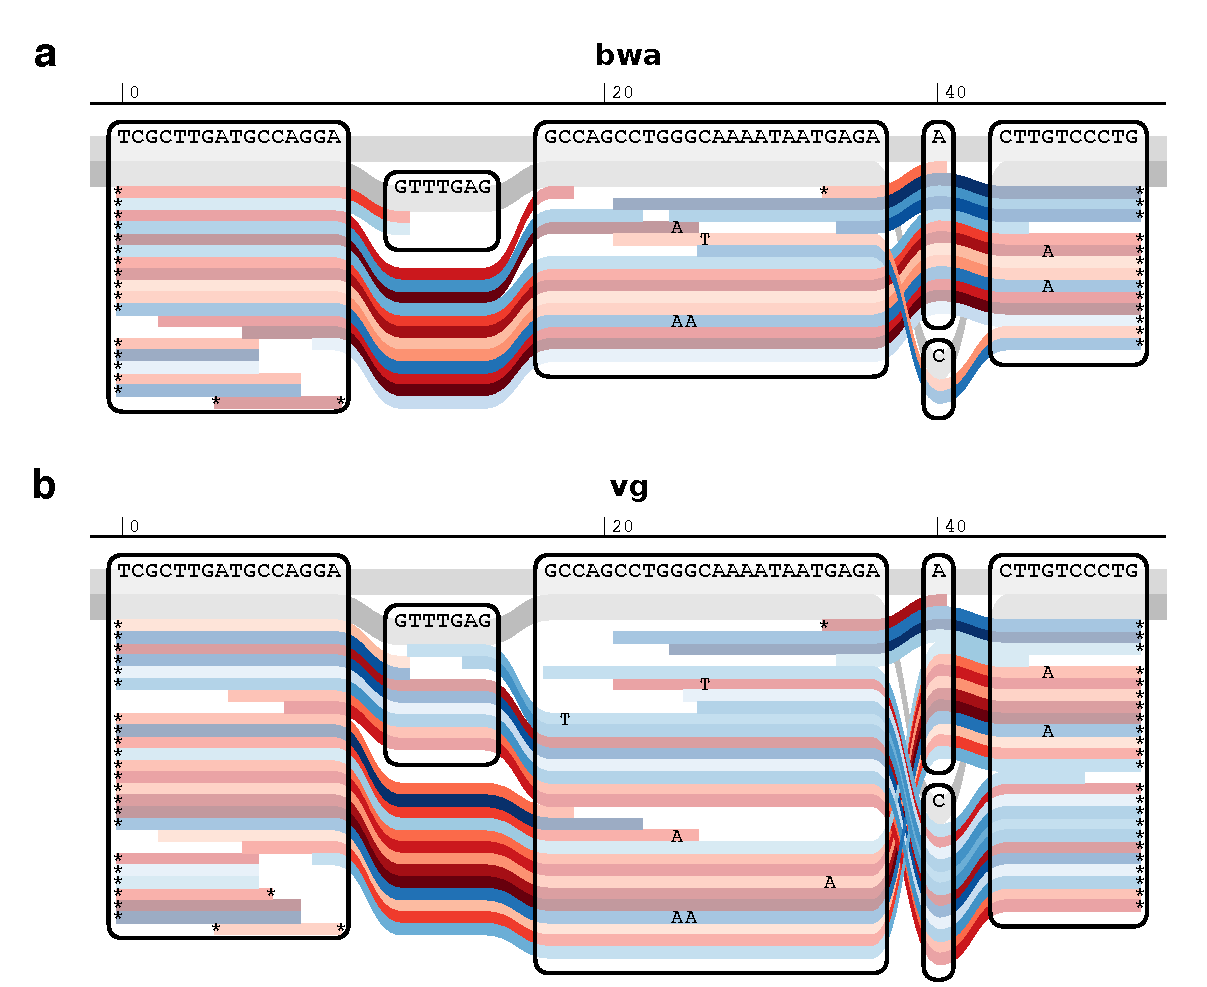
\includegraphics[width=0.95\textwidth]{tubemap.pdf}
\vspace{-8pt}
\captionof{figure}{Sequence tube maps of a small region of the human genome with aDNA reads from the Yamnaya individual aligned with A) {\tt bwa aln} to a linear reference sequence and B) {\tt vg map} to a graph containing 1000 Genomes variants.}
\end{center}
The individual is heterozygous for both an indel (GTTTGAG/-) and a SNP (A/C) in this region, with insertion and alternate allele on the same haplotype. The two underlying haplotypes in this region are coloured in grey, and red and blue lines indicate forward and reverse reads respectively. None of the 6 reads across the insertion and only 2 of 12 reads across the SNP were mapped by \bwa. 
}

%----------------------------------------------------------------------------------------
%	RESULTS
%----------------------------------------------------------------------------------------

\headerbox{Simulated ancient DNA data}{name=sims,span=1,column=2,row=0, above dstats}{ % To reduce 

%  \begin{center}
%   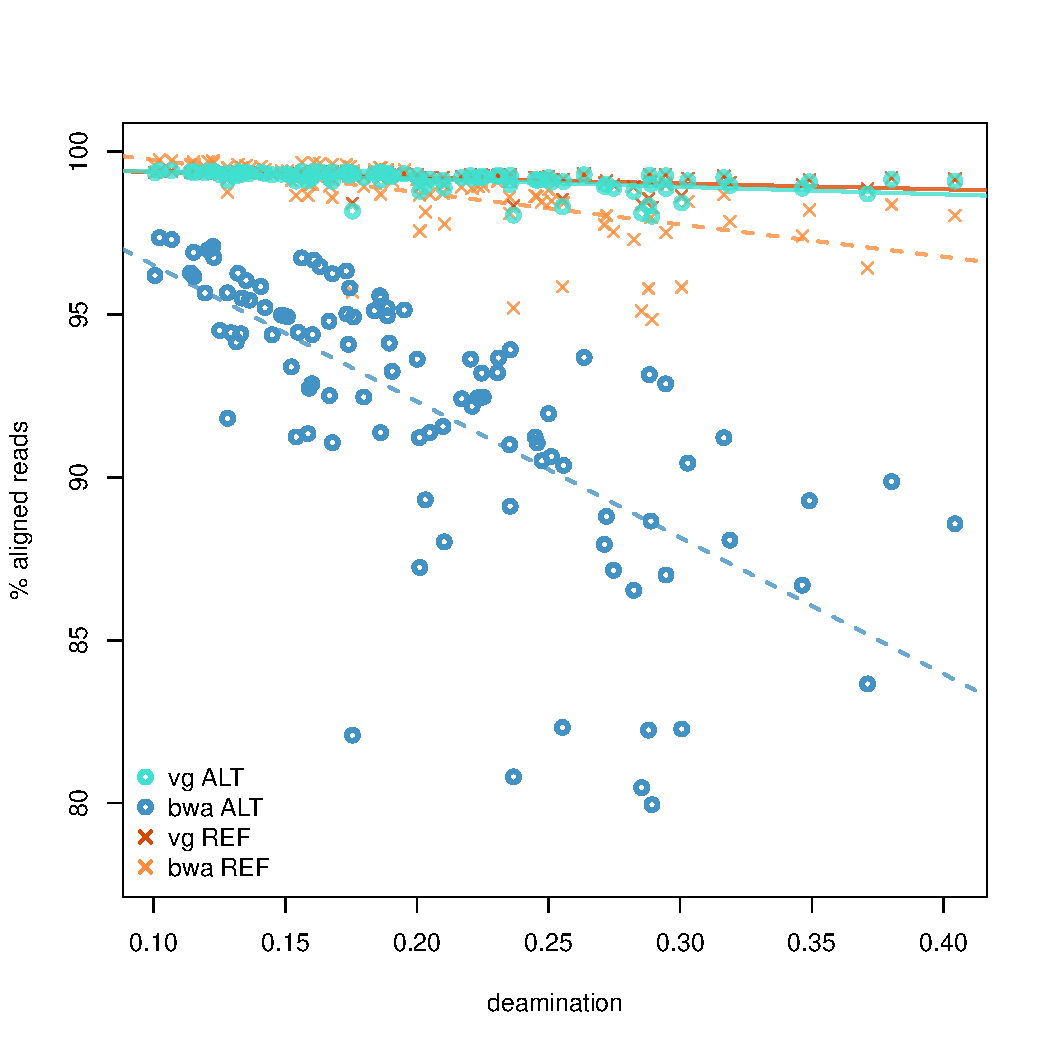
\includegraphics[width=0.95\textwidth]{main_fig_percent_aln.pdf}
% \vspace{-8pt}
% \captionof{figure}{Comparing {\tt bwa aln} (mapping quality 30) and {\tt vg map} (mapping quality 50) performance when aligning reads simulated from chromosome 11 of the Human Origins panel.
%     Lines represent ordinary least squares (OLS) regression results for the allele/aligner conditions corresponding to their colors.}
% \end{center}

 \begin{center}

  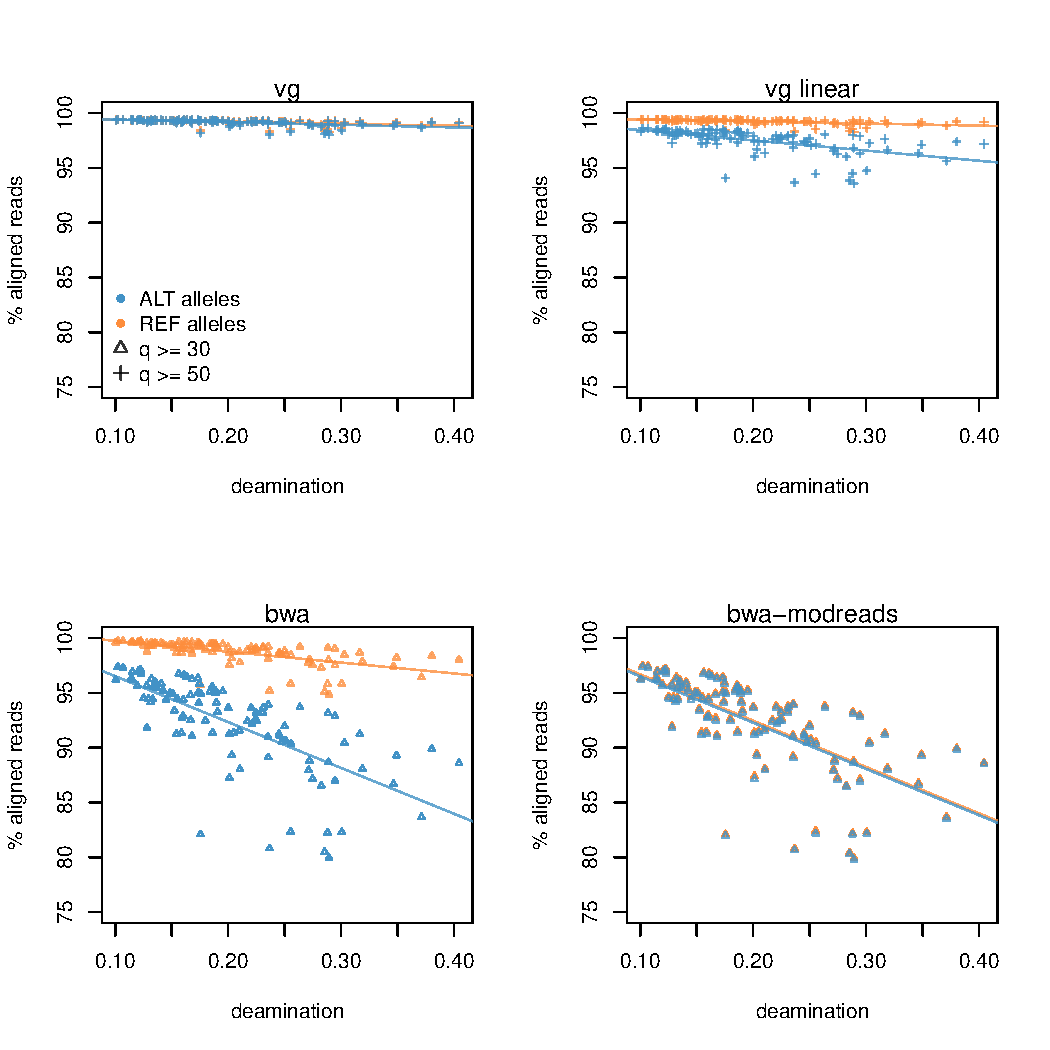
\includegraphics[width=0.95\textwidth]{percent_aln_split_2cols_simplified_w_modreads.pdf}
\captionof{figure}{Comparison of the percentage of mapped reads in simulated data between bwa, bwa-modreads) (mapping quality filter q$\geq$30), vg graph and vg linear reference (q$\geq$50).}

\end{center}

At high levels of simulated damage, alignment with \bwa{} against the linear reference prevents the observation of non-reference alleles in a large fraction of cases. In contrast there is no such reduction for {\tt vg map}.
\\
In the \vg{} alignment to the linear reference, similarly to \bwa{}, the percentage of aligned reads with the alternate allele drops as deamination increases.
\\
We also applied the read modification protocol of Gunther et al. to our \bwa{} mapping data. In this case, the bias is removed, but at the cost of a substantial decrease in sensitivity for reads containing the reference as well as alternate alleles.



}




%----------------------------------------------------------------------------------------
%	RESULTS
%----------------------------------------------------------------------------------------


\headerbox{Downsampling experiment.}{name=downsampling,span=1,column=1,below=tubemap}{ 


 \begin{center}
  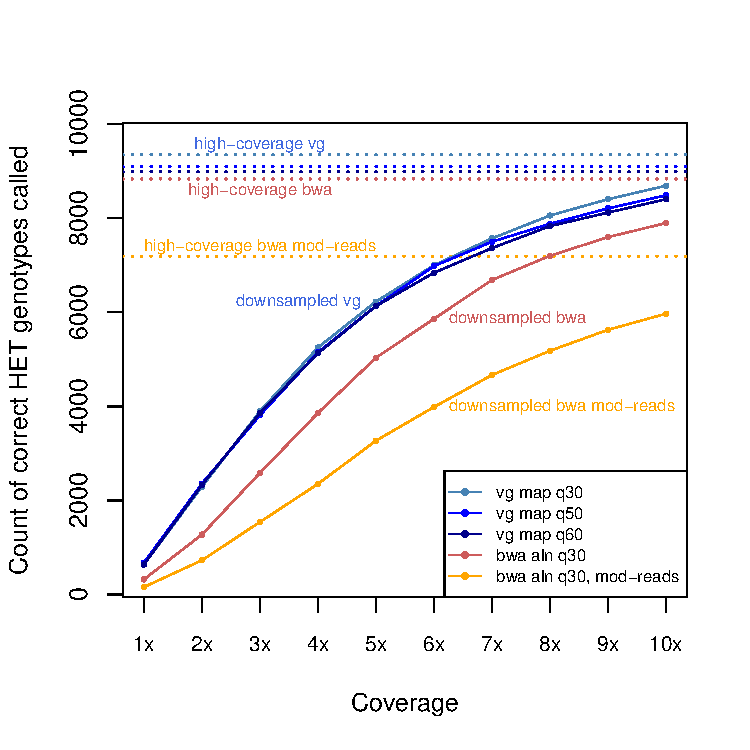
\includegraphics[width=0.95\textwidth]{mainfig_downsampling_exp.pdf}
\vspace{-8pt}
\captionof{figure}{The comparative effect of downsampling on heterozygous variant calling following {\tt bwa aln} and {\tt vg map} alignment of reads from the ancient Yamnaya sample, including post-processing of {\tt bwa aln} with the modified read filter.}
\end{center}

We next measured our ability to recover the heterozygous variants in the full coverage set at lower coverage levels. {\tt bwa aln} recovers fewer heterozygous SNPs than {\tt vg map} alignment to the 1000GP graph at all coverage levels. For example at 4x coverage, {\tt vg map} recovers $\approx$13\% more heterozygotes as a fraction of the total. Filtering \bwa{} alignments using read modification (Torsten et al., 2019) reduces sensitivity still further. 


}

\headerbox{Alignment accuracy}{name=test,span=1,column=1,below=downsampling}{ 
\tiny{\textbf{Table 2}. \vg{} graph mapping to the graph (q50) and \bwa{} (q30) have comparable read mapping accuracy. \vg{} linear mapping is less accurate.}
\begin{table}[H]
\centering


\resizebox{\textwidth}{!}{%
\begin{tabular}{cccccccccc}
\hline
\multirow{2}{*}{\textbf{\begin{tabular}[c]{@{}c@{}}mapping\\ quality threshold\end{tabular}}} & \multicolumn{3}{c}{\textbf{mean error REF (\%)}} & \multicolumn{3}{c}{\textbf{mean error ALT (\%)}} & \multicolumn{3}{c}{\textbf{mean error All (\%)}} \\ \cline{2-10} 
 & \textbf{vg} & \textbf{vg linear} & \textbf{bwa} & \textbf{vg} & \textbf{vg linear} & \textbf{bwa} & \textbf{vg} & \textbf{vg linear} & \textbf{bwa} \\ \hline
\textbf{q\textgreater{}=30} & 0.00015 & 0.00017 & 0.00002 & 0.00037 & 0.00162 & 0.00024 & 0.00026 & 0.00089 & 0.00012 \\
\textbf{q\textgreater{}=50} & 0.00012 & 0.00013 & - & 0.00025 & 0.00110 & - & 0.00019 & 0.00061 & - \\
\textbf{q\textgreater{}=60} & 0.00011 & 0.00012 & - & 0.00021 & 0.00097 & - & 0.00016 & 0.00054 & - \\ \hline
\end{tabular}%
}
\end{table}
}
% \headerbox{Contact}{name=contact,span=1,column=1,below=downsampling,above=bottom}{ 

%  \begin{center}
%  rm890@cam.ac.uk
%  \end{center}

%  }

%----------------------------------------------------------------------------------------
%	RESULTS
%----------------------------------------------------------------------------------------



      
\headerbox{$D$-statistics}{name=dstats,span=1,column=2,below=sims,above=bottom}{ 

 \begin{center}
  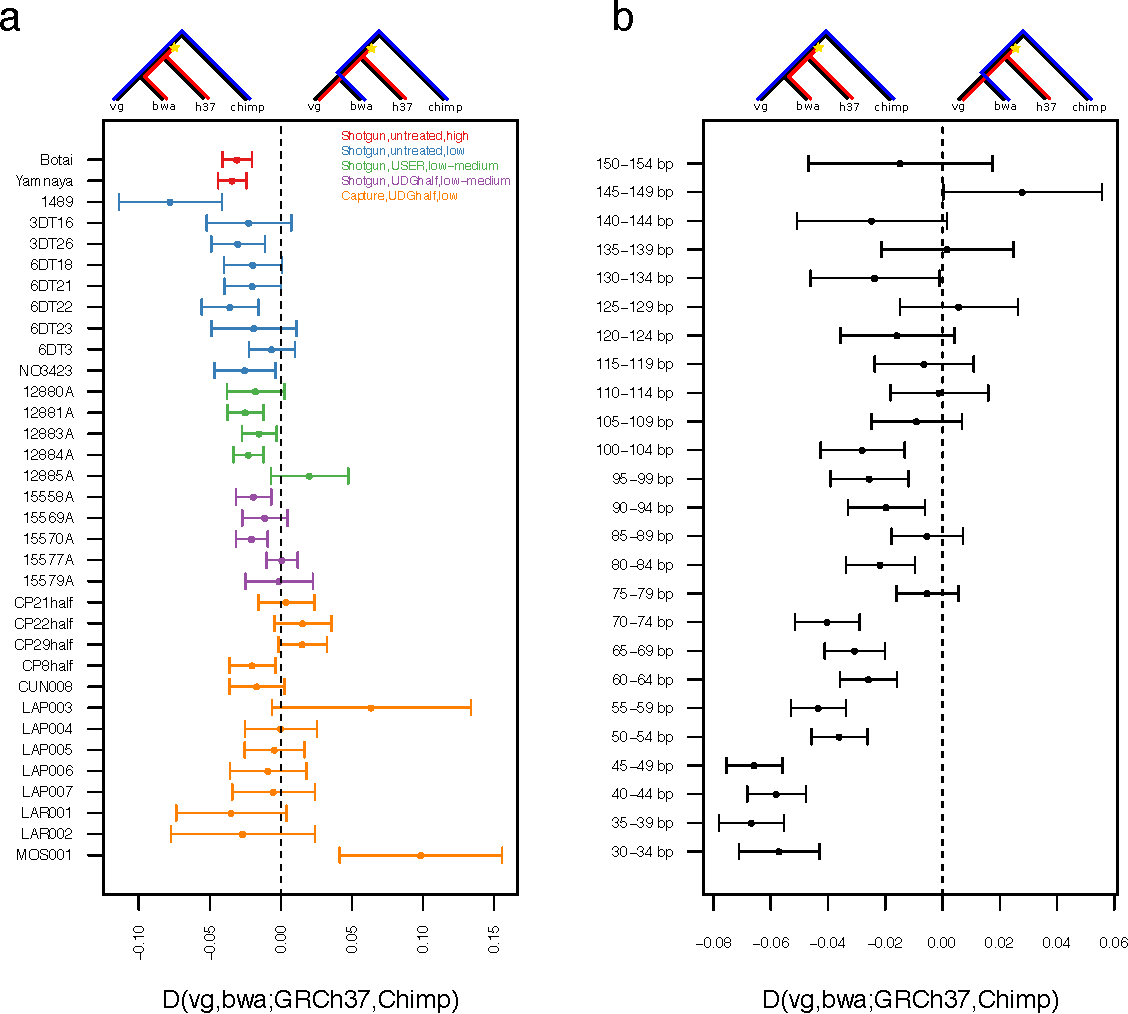
\includegraphics[width=0.95\textwidth]{new_mainfig_dstats_diag.pdf}
\vspace{-8pt}
\captionof{figure}{$D$-statistic of the form $D$(vg, bwa; GRCh37, Chimp) to test reference bias in aDNA. a) $D$-statistics estimated for 34 ancient individuals, using transversion SNPs only. The figure label indicates the type of sequencing, enzymatic treatment and genomic coverage for each sample. b) $D$-statistic for the ancient Yamnaya sample stratified by read length.
}
\end{center}

Our results show negative $D$-statistics for all but a handful of samples, consistent with \bwa{} calls being closer to the reference than \vg{} calls. The bias in D statistic between \vg{} and \bwa{} is strongest for shorter reads, as seen when we stratify the data by read length as in Figure 4b and as previously reported (Gunther, 2019).

}


\end{poster}

\end{document}